\section{Outlier detection}
\label{sec:functional_outlier}

\begin{figure}
    \centering
    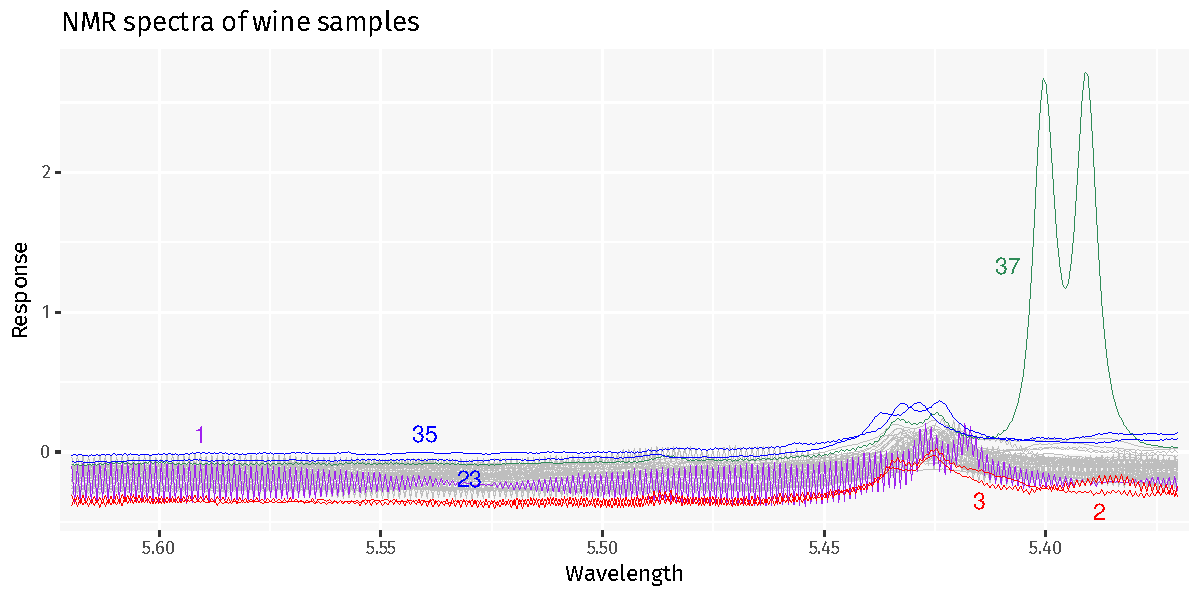
\includegraphics[width = \textwidth]{wine}
    \caption{
        NMR spectra of 40 wine samples\protect\footnotemark, from the R
        package \texttt{speaq}, with some curves showing outlying behaviour
        highlighted.
        The green curve \#37 is an isolated outlier, the blue and red curves
        are shift outliers, and the purple curve is a shape outlier.
    }
    \label{fig:wine}
\end{figure}
\footnotetext{\url{https://ucphchemometrics.com/datasets/}}

A curve $\vx\colon [0, 1] \to \R$ may exhibit outlying behaviour with respect
to a body of curves in many ways; we use the useful classification as detailed
in \textcite{hubert-rousseeuw-segeart-2015}.
It may deviate significantly over a short interval, in which case we call it
an \emph{isolated outlier}.
Alternatively, it may deviate over a large, or perhaps even the whole
interval, in which case we call it a \emph{persistent outlier}.
If this deviation is in terms of shape -- for instance, the curve may be
rougher or smoother -- we call it a \emph{shape outlier}.
Otherwise, if the curve has the same shape as the rest but appears above or
below them, we call it a \emph{shift outlier}.
Another possibility is that the curve differs in scale, in which case we call
it an \emph{amplitude outlier}.
Some of these behaviours have been illustrated in the dataset in
Figure~\ref{fig:wine}.

An important consideration when dealing with shape outliers is that each time
slice $\vx(t)$ may be fairly inconspicuous with respect to the marginal
$F_{\vX(t)}$.
Thus, it seems clear that a tool like the Fraiman-Muniz depth may succeed in
identifying shift or amplitude outliers, but fall short against shape
outliers.
In general, the basic algorithm of iteratively selecting curves with low
functional depth as outliers is often insufficient.

A common approach towards examining the shapes of curves in a dataset is to
bundle them with their derivatives.
For instance, motion data often involves tracking both position and velocity
over time.
Thus, one may replace a curve $x$ by $(x(\Cdot), x'(\Cdot))$ and examine its
depth; the Fraiman-Muniz depth for such a curve would be of the form
\begin{equation}
    D_F^{(2)}(x, F_{X}) = \int_{[0, 1]} D((x(t), x'(t))^\top, F_{(X(t), X'(t))^\top}) \:w(t)\:dt.
\end{equation}
This naturally extends to $D_F^{(J)}$, taking derivatives of order $0, \dots,
J - 1$.
\textcite{nagy-gijbels-hlubinka-2017} point out several difficulties with this
formulation, primarily the assumption of differentiability and the errors
introduced when approximating derivatives.
They make the notion of a $J$-th order shape outlier more precise as follows.

\begin{definition}
    If there exists $\bm{t} \in [0, 1]^J$ such that $(\vx(t_1), \dots,
    \vx(t_J))^\top$ is outlying with respect to $F_{(\vX(t_1), \dots,
    \vX(t_J))^\top}$, then we say that $\vx$ is a $J$-th order outlier with
    respect to $F_{\vX}$.
\end{definition}

With this, the $J$-th order extension of Fraiman Muniz depth
(Definition~\ref{def:J_FM_depth}) is well equipped to detect $J$-th order
outliers.
\textcite{nagy-gijbels-hlubinka-2017} show that this depth $D_F^J$
incorporates information about the $J$-th order derivatives of the curves
(along with potentially additional information about its shape), which makes
its performance comparable to or even better than $D_F^{(J)}$.
They supply a simple algorithm based on $D_F^J$ values for identifying $J$-th
order outliers.
A similar argument can be made for the $J$-th order extension of the infimal
depth (Definition~\ref{def:J_Inf_depth}).


\subsection{Outliergrams}

\begin{figure}
    \centering
    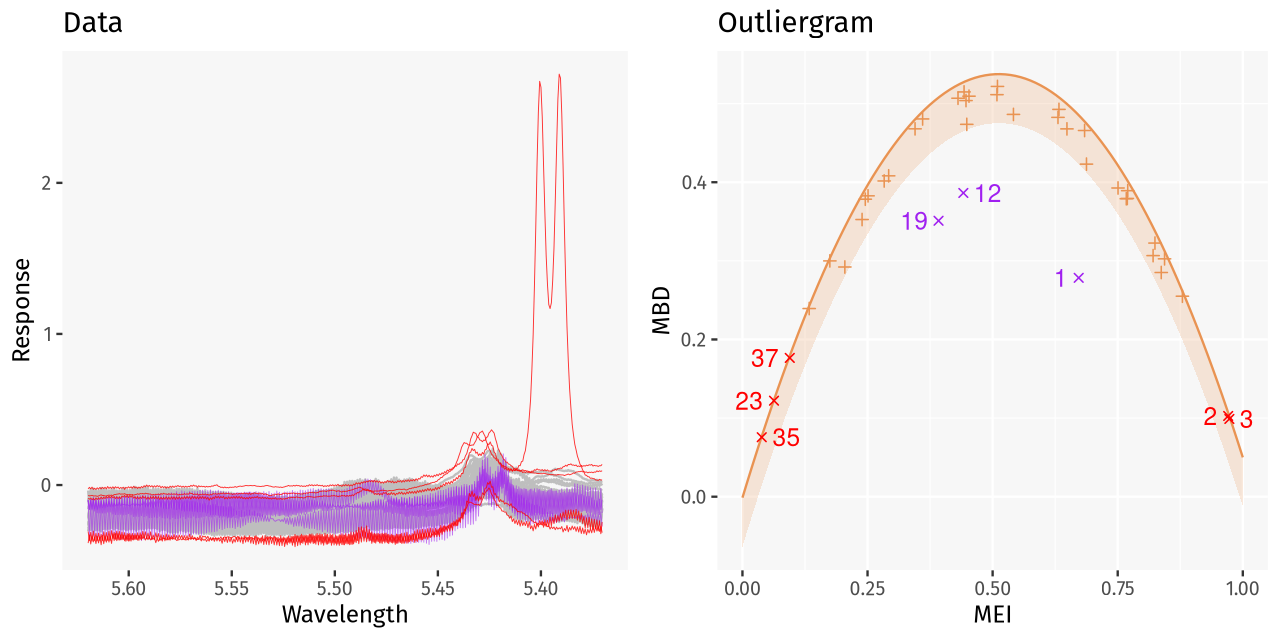
\includegraphics[width = \textwidth]{outliergram_wine}
    \caption{
        Outliergram for the NMR spectra of 40 wine samples.
        The three purple curves have been identified as shape outliers, as
        they fall outside the orange ribbon in the outliergram.
        Although the red curves lie on the orange parabola, they have low MBD
        and extreme MEI values, indicating that they lie above or below the
        main mass of curves.
    }
    \label{fig:outliergram_wine}
\end{figure}


\textcite{gil-romo-2014} combined the notions of the modified epigraph index
(MEI) and the modified band depth (MBD), proposing the outliergram as a tool
for detecting shape outliers.
They show that for a sample $\{\vx_i\}_{i = 1}^n$, each
\begin{equation}
    \MBD(\vx_i) = D_{MB}(\vx_i, \hat{F}_n) \leq a_0 + a_1 \MEI(\vx_i) + a_2 n^2 \MEI(\vx_i)^2
\end{equation}
where $a_0 = a_2 = -2/n(n - 1)$ and $a_1 = 2(n + 1)/(n - 1)$.
The distance
\begin{equation}
    d_i = a_0 + a_1 \MEI(\vx_i) + a_2 n^2 \MEI(\vx_i) - \MBD(\vx_i)
\end{equation}
is indicative of the outlyingness of $\vx_i$.
\textcite{gil-romo-2014} consider shape outlying curves as those for which
$d_i \geq d^* = Q_3 + 1.5\IQR$, where $Q_3$ and $\IQR$ are the third quartile
and the interquartile range of $\{d_i\}_{i = 1}^n$ respectively.

\begin{definition}[Outliergram]
    The outliergram for a dataset $\mathscr{D} = \{\vx_i\}_{i = 1}^n$ is the
    graph
    \begin{equation}
        \{(\MEI(\vx_i, \hat{F}_n),\, \MBD(\vx_i, \hat{F}_n))\colon 1 \leq i \leq n\}.
    \end{equation}
    Shape outliers are curves $\vx_i$ such that $(\MEI_i, \MBD_i)$ falls
    outside a ribbon of height $d^*$ under the parabola $a_0 + a_1 \MEI +
    a_2n^2\MEI^2$.
\end{definition}

Figure~\ref{fig:outliergram_wine} illustrates the use of the outliergram.
We have also highlighted curves with fairly low or high MEI values as shift
outliers; a low MEI value indicates that the curve lies above the main mass of
curves, and a high MEI indicates that it lies below.


\subsection{Centrality-Stability diagrams}

\begin{figure}
    \centering
    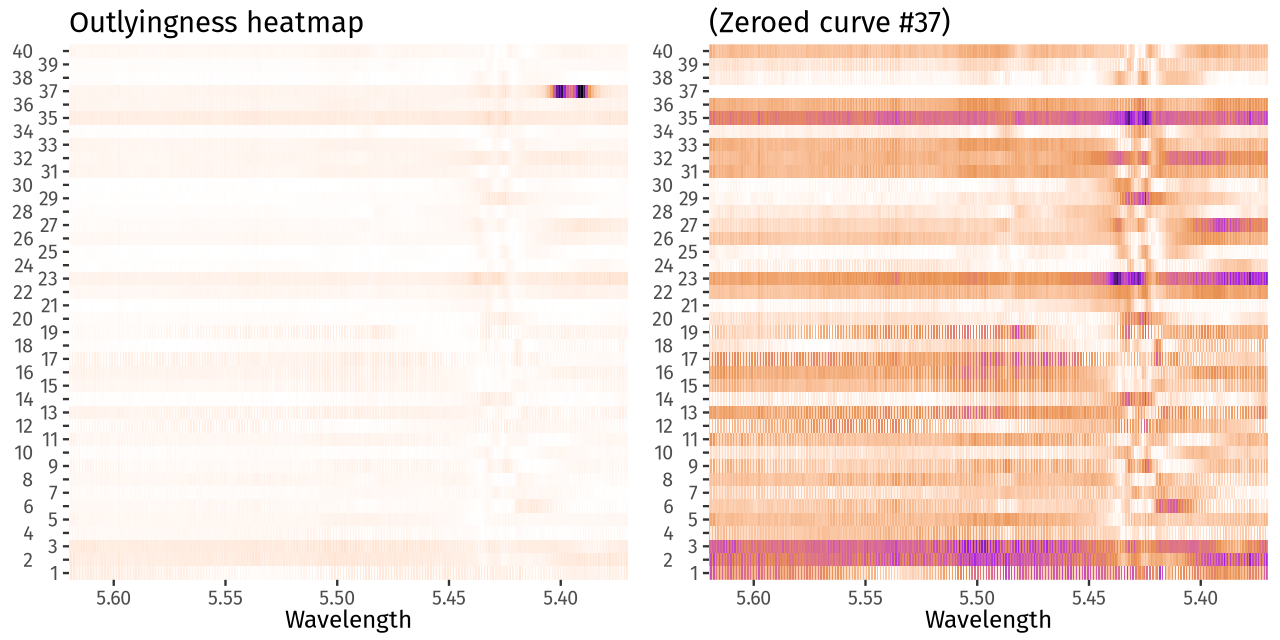
\includegraphics[width = \textwidth]{outlyingness_heatmap_wine}
    \caption{
        Outlyingness heatmap for the NMR spectra of 40 wine samples.
        The extreme curve \#37 has been zeroed out in the second diagram to
        better illustrate the variation in outlyingness for the remaining
        curves.
    }
    \label{fig:outlyingness_heatmap_wine}
\end{figure}

\begin{figure}
    \centering
    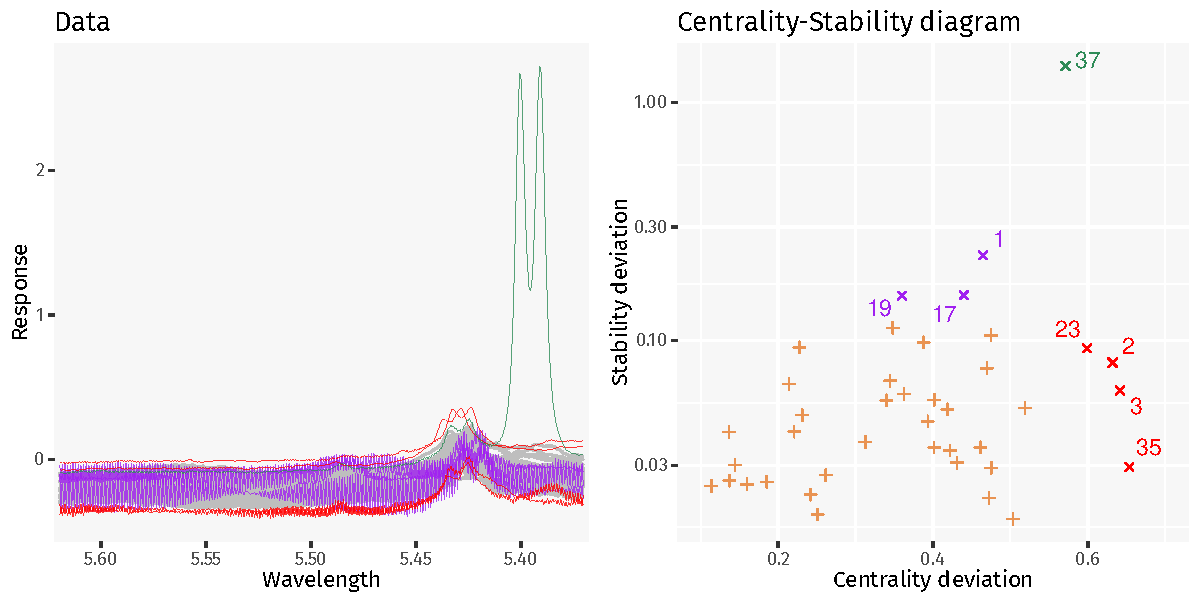
\includegraphics[width = \textwidth]{centrality_stability_wine}
    \caption{
        Centrality-Stability diagram for the NMR spectra of 40 wine samples.
        The red curves are seen to deviate in terms of centrality, indicated
        by the fact that the corresponding points in the centrality-stability
        diagram fall towards the right.
        The purple curves deviate in terms of stability, with the green curve
        showing extreme deviation.
    }
    \label{fig:centrality_stability_wine}
\end{figure}

In their discussion of methods of functional outlier detection,
\textcite{hubert-rousseeuw-segeart-2015} proposed the centrality-stability
diagram, where both the `centrality' of a curve (measured by depth) and its
variability in cross-sectional outlyingness over time are accounted for.
A deviation in centrality may point towards a shift outlier, while a deviation
in stability may point towards an isolated or shape outlier.

\textcite{hubert-rousseeuw-segeart-2015} begin by choosing a multivariate
depth function of the form $D'(\vx(t), F_{\vX(t)}) = (1 + O(\vx(t)))^{-1}$,
where $O(\Cdot)$ is an outlyingness function.
The Mahalanobis, projection, and Oja depths clearly fit this description.
Here, for the purposes of computation in the univariate case, we choose
\begin{equation}
    O(x(t)) = \frac{|x(t) - \med(X(t)|}{\MAD(X(t))},
\end{equation}
instead of using the skew-adjusted version; the differences are minor enough
for us to ignore.
The variation in $O(\vx(\Cdot))$ over time for different curves, in the form
of an \emph{outlyingess heatmap}, is quite revealing;
Figure~\ref{fig:outlyingness_heatmap_wine} shows that curves may have large
outlyingness for short or long intervals.

Corresponding to $D'$, we have an integrated Fraiman-Muniz depth
\begin{equation}
    D_F(\vx, F) = \int_{[0, 1]} (1 + O(\vx(t)))^{-1}\:dt.
\end{equation}
However, a spike in outlyingess over a short time interval, such as in curve
\#37 in Figure~\ref{fig:outlyingness_heatmap_wine}, may potentially be `washed
out' in this averaging.
With this, we seek a method of detecting sharp bursts in outlyingness.
Note that by setting
\begin{equation}
    \widetilde{\MOt}(\vx, F) = \int_{[0, 1]} O(\vx(t)) \:dt,% = \int_{[0, 1]} \left(\frac{1}{D'(\vx(t), F_{\vX(t)})} - 1\right) \:dt,
\end{equation}
Cauchy-Schwarz gives us the relation
\begin{equation}
    D_F(\vx, F) \Cdot (1 + \widetilde{\MOt}(\vx, F)) \geq 1.
\end{equation}
Equality is achieved only when $O(\vx(\Cdot))$ remains constant over time.
Any sudden variation in outlyingness over time will be detected by the
\emph{stability deviation}
\begin{equation}
    \Delta S(\vx, F) \;=\; (1 + \widetilde{\MOt}(\vx, F)) - \frac{1}{D_F(\vx, F)},
\end{equation}
the difference between the arithmetic and harmonic means of $1 +
O(\vx(\Cdot))$.
Defining the \emph{centrality deviation} simply as $\Delta C(\vx, F) = 1 -
D_F(\vx, F)$, we have our \emph{centrality-stability diagram}.

\begin{definition}[Centrality-Stability diagram]
    The centrality-stability diagram for a dataset $\mathscr{D} = \{\vx_i\}_{i
    = 1}^n$ is the graph
    \begin{equation}
        \{(\Delta C(\vx_i, \hat{F}_n),\, \Delta S(\vx_i, \hat{F}_n))\colon 1 \leq i \leq n\}.
    \end{equation}
\end{definition}

\begin{remark}
    We make a distinction between $\MO$ from Definition~\ref{def:MO} and
    $\widetilde{\MOt}$; the outlyingness $O(\Cdot)$ used in the latter is real
    and positive.
\end{remark}

Figure~\ref{fig:centrality_stability_wine} illustrates the use of the
centrality-stability diagram as a summary of the outlyingness heatmap from
Figure~\ref{fig:outlyingness_heatmap_wine}.
This time, the isolated outlier curve \#37 is well separated from the shift
and shape outliers, unlike in the outliergram in
Figure~\ref{fig:outliergram_wine}.




\subsection{MO-VO diagrams}

\begin{figure}
    \centering
    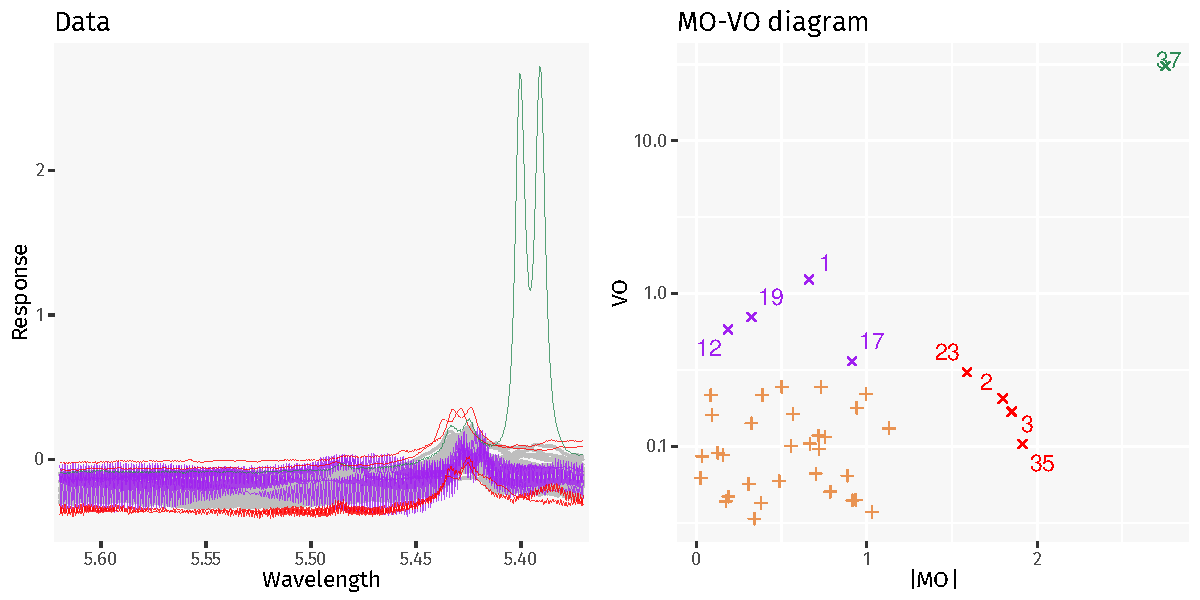
\includegraphics[width = \textwidth]{MO_VO_wine}
    \caption{
        MO-VO diagram for the NMR spectra of 40 wine samples.
        We plot $|\MOt|$ rather than MO here for better comparison with the
        centrality stability diagram in
        Figure~\ref{fig:centrality_stability_wine}; nevertheless, the signed
        MO values would reveal whether the shift outliers lie above or below
        the main mass of curves.
    }
    \label{fig:MO_VO_wine}
\end{figure}

We observe that the MO-VO diagram from \textcite{dai-genton-2018} neatly falls
under a general category of centrality-stability diagrams.
The quantity $\MO(\vx, F)$ may indeed be treated as a measure of deviation
from centrality of $\vx$.
Again, $\VO(\vx, F)$ being the variance of $\vO(t)$, may be treated as a
measure of deviation from stability, since it captures the variability of
outlyingness over time and is sensitive to changes over short intervals.

\begin{definition}[MO-VO diagram]
    The MO-VO diagram for a dataset $\mathscr{D} = \{\vx_i\}_{i = 1}^n$ is the
    graph
    \begin{equation}
        \{(\MO(\vx_i, \hat{F}_n),\, \VO(\vx_i, \hat{F}_n))\colon 1 \leq i \leq n\}.
    \end{equation}
\end{definition}


For the purposes of computation in the univariate case, we use the directional
outlyingess function
\begin{equation}
    O(x(t)) = \frac{x(t) - \med(X(t))}{\MAD(X(t))}.
\end{equation}
Figure~\ref{fig:MO_VO_wine} illustrates the use of the MO-VO diagram.
Note the similarities with the centrality-stability diagram from
Figure~\ref{fig:centrality_stability_wine}.




\begin{figure}
    \centering
    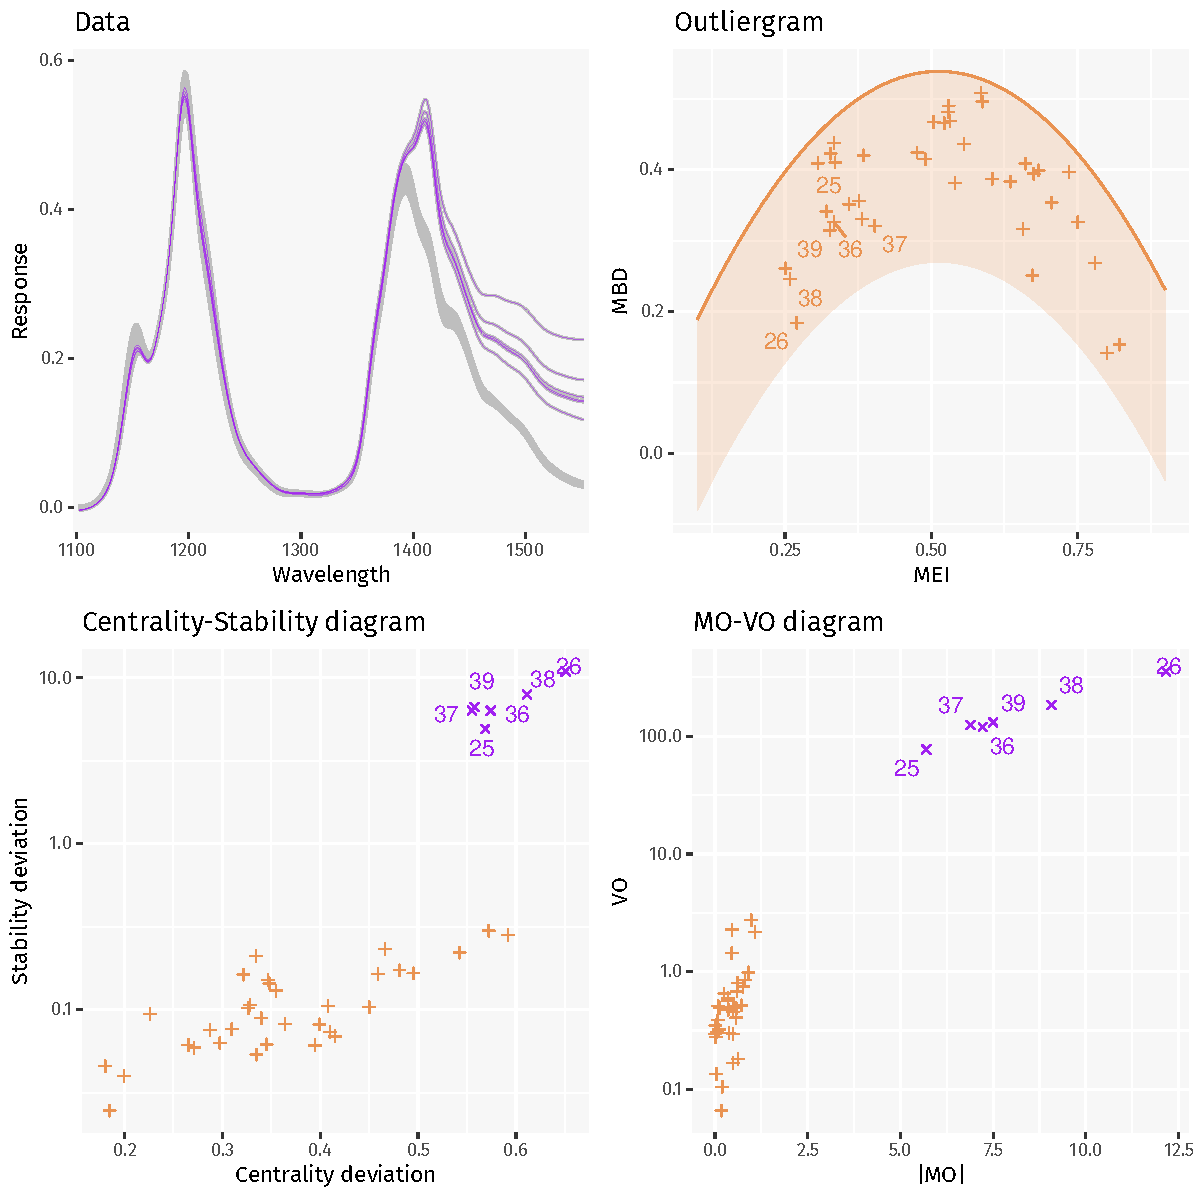
\includegraphics[width = \textwidth]{outlyingness_octane}
    \caption{
        Outliergram, centrality-stability, and MO-VO diagrams for the NIR
        spectra of 39 gasoline samples, from the R package \texttt{rrcov}.
        The six purple curves \#25, 26, 36-39 correspond to samples containing
        added alcohol.
        While the outliergram does not clearly identify these outliers, the
        centrality-stability and MO-VO diagrams show a marked separation from
        the main curves.
        Indeed, there is no cutoff $d^*$ defining the lower boundary of the
        orange ribbon in the outliergram which properly excludes the six
        outliers.
    }
    \label{fig:outlyingness_octane}
\end{figure}

\begin{figure}
    \centering
    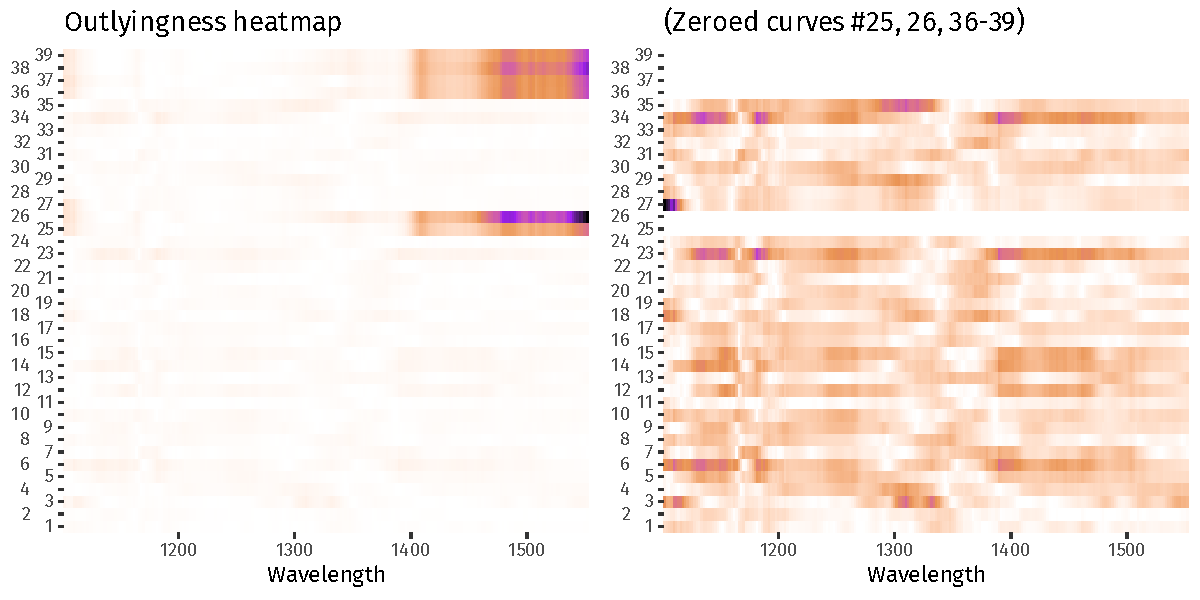
\includegraphics[width = \textwidth]{outlyingness_heatmap_octane}
    \caption{
        Outlyingness heatmap for the NIR spectra of 39 gasoline samples.
        The outlying curves have been zeroed out in the second diagram.
    }
    \label{fig:outlyingness_heatmap_octane}
\end{figure}


We demonstrate all of the above diagnostic tools on a different dataset in
Figures~\ref{fig:outlyingness_heatmap_octane} and
\ref{fig:outlyingness_octane}.
